\documentclass{standalone}
\usepackage{tikz}
\usetikzlibrary{cd, arrows.meta, positioning}
\usepackage{amsmath, amssymb}

\begin{document}
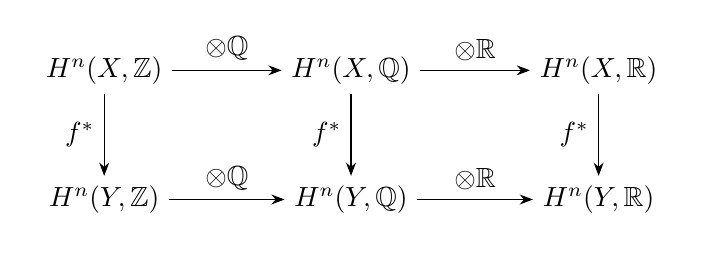
\begin{tikzpicture}
  \matrix (m) [matrix of math nodes, row sep=3em, column sep=4em, minimum width=2em] {
    H^n(X, \mathbb{Z}) & H^n(X, \mathbb{Q}) & H^n(X, \mathbb{R}) \\
    H^n(Y, \mathbb{Z}) & H^n(Y, \mathbb{Q}) & H^n(Y, \mathbb{R}) \\
  };

  % Horizontal arrows
  \path[-Stealth]
    (m-1-1) edge node [above] {$\otimes \mathbb{Q}$} (m-1-2)
    (m-1-2) edge node [above] {$\otimes \mathbb{R}$} (m-1-3)
    (m-2-1) edge node [above] {$\otimes \mathbb{Q}$} (m-2-2)
    (m-2-2) edge node [above] {$\otimes \mathbb{R}$} (m-2-3);

  % Vertical arrows
  \path[-Stealth]
    (m-1-1) edge node [left] {$f^*$} (m-2-1)
    (m-1-2) edge node [left] {$f^*$} (m-2-2)
    (m-1-3) edge node [left] {$f^*$} (m-2-3);
\end{tikzpicture}
\end{document}
